% ===================================================================
\section{Results}\label{sec:results}
% ===================================================================
\subsection{Pre-event fit}
Table~\ref{tab:wfcv} reports walk-forward cross-validation. The pattern matches the two
events' pre-periods. For Hormuz, whose pre-period is calm, four of five models clear the
heuristic overfit flag and the fifth sits only just past it. For Russia, whose pre-period
spans the volatile 2020--22 recovery, more models trip the flag, because a noisy
pre-period inflates validation error. The flags do not exclude any model. They mark which
synthetics to read with more caution, and the headline outlier in each event
is among the flagged models, so the flags and the outlier tell a consistent story.

\begin{table}[h]
\centering
\caption{Walk-forward cross-validation (5 expanding folds, 20-day horizons). A
validation/training RMSE ratio above 2 is a heuristic overfit flag, not an exclusion rule.}
\label{tab:wfcv}
\small
\begin{tabular}{@{}llrl@{}}
\toprule
Event & Model & val/train RMSE & Flag \\
\midrule
Russia & Convex SCM     & 1.25 & OK \\
Russia & Augmented SCM  & 2.06 & overfit \\
Russia & Elastic net    & 1.99 & OK \\
Russia & XGBoost        & 3.24 & overfit \\
Russia & Bayesian ridge & 3.09 & overfit \\
\addlinespace
Hormuz & Convex SCM     & 1.40 & OK \\
Hormuz & Augmented SCM  & 1.54 & OK \\
Hormuz & Elastic net    & 1.51 & OK \\
Hormuz & XGBoost        & 1.84 & OK \\
Hormuz & Bayesian ridge & 2.28 & overfit \\
\bottomrule
\end{tabular}
\end{table}

\subsection{Headline estimates}
Table~\ref{tab:headline} reports the per-model post-window gap and the drift-adjusted gap
for both events, and Figure~\ref{fig:paths} plots the observed and synthetic paths. For
\textbf{Russia 2022} the ensemble-median premium is \SI{22.0}{\percent} over the
seven-month window (IQR \SIrange{10.9}{30.8}{\percent}), which implies a counterfactual
mean of \$88.6/bbl against an actual \$108.5. This is consistent with the documented
\$95$\to$\$130 move and its partial reversion by September. For \textbf{Hormuz 2026} the
ensemble-median premium is \SI{55.9}{\percent} over the window to mid-June (IQR
\SIrange{51.2}{56.6}{\percent}), with an actual post-window mean of \$106.9 against an
implied counterfactual near \$68.6. The Hormuz band is far tighter than Russia's, about
5 points against about 20, which reflects the calmer Hormuz pre-period.

\begin{table}[h]
\centering
\caption{Headline post-event gaps (\%). Drift-adjusted $=$ raw gap minus the pre-period
gap trend extrapolated over the post-window (see Section~\ref{sec:methods}). Ensemble $=$
cross-model median, band $=$ IQR (Q25--Q75).}
\label{tab:headline}
\small
\begin{tabular}{@{}lrr@{\hskip 1.6em}rr@{}}
\toprule
& \multicolumn{2}{c}{Russia 2022 (7 mo)} & \multicolumn{2}{c}{Hormuz 2026 ($\sim$3.5 mo)}\\
\cmidrule(lr){2-3}\cmidrule(lr){4-5}
Model & Raw & Adj. & Raw & Adj. \\
\midrule
Convex SCM     & 33.6 & 28.4 & 55.9 & 57.3 \\
Augmented SCM  & 10.9 & 10.6 & 56.8 & 57.1 \\
Elastic net    & 22.0 & 21.2 & 56.6 & 57.4 \\
XGBoost        & 30.8 & 28.9 & 51.2 & 52.7 \\
Bayesian ridge & $-9.0$ & $-9.1$ & 43.0 & 43.0 \\
\midrule
\textbf{Ensemble median} & \textbf{22.0} & \textbf{21.2} & \textbf{55.9} & \textbf{57.1} \\
\textbf{IQR} & \textbf{[10.9, 30.8]} & n/a & \textbf{[51.2, 56.6]} & n/a \\
\bottomrule
\end{tabular}
\end{table}

\begin{figure}[h]
\centering
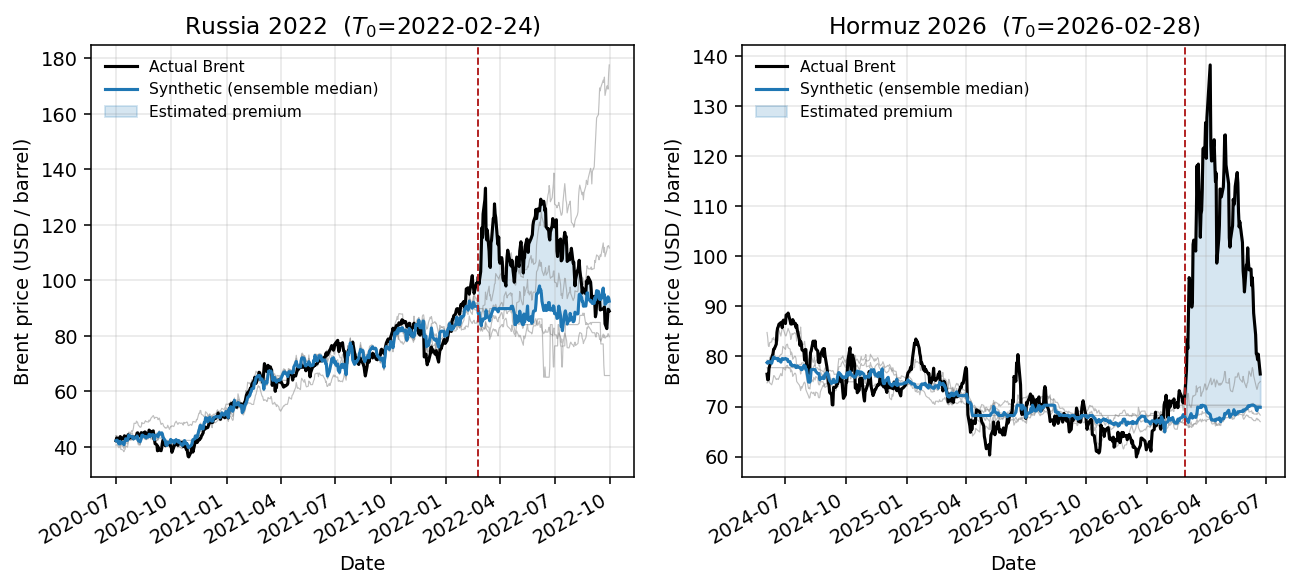
\includegraphics[width=\textwidth]{figures/counterfactual_paths.png}
\caption{Observed Brent (black) vs.\ the synthetic counterfactual. The thick blue line
is the ensemble-median synthetic, thin grey lines are the five individual models, and the
shaded region after $T_0$ (dashed red) is the estimated premium. The synthetics track
Brent closely before the event and decouple sharply afterward.}
\label{fig:paths}
\end{figure}

\paragraph{Economic reading of the model spread.} The cross-model dispersion has an
economic explanation rather than reflecting noise, and this is the one place where the
individual models matter, so we name them here. Convex SCM, confined to the simplex,
leans on the most stable donors, the FX block, as a trend baseline and adds
soft-commodity deltas such as Coffee and Sugar for Russia. The Bayesian ridge, with
unconstrained Gaussian coefficients, loads heavily and with large opposing signs on
currencies. For Russia those currencies moved with the simultaneous and historically
large Fed tightening cycle, a macro factor that has nothing to do with the invasion. That
confound is why the Bayesian ridge becomes the Russia outlier, with a negative full-window
gap, and why it carries a high walk-forward flag. It is the expected behaviour of an
unregularised linear model in a pre-period that contains a strong non-event driver, and it
is the reason the ensemble uses the median rather than the mean. For Hormuz, whose calmer
pre-period has no analogous confound, the five models agree to within about 5 points.

\subsection{Donor contributions}
To understand why the Russia ensemble is dispersed while Hormuz is comparatively
concentrated, we look at the donor contributions behind each model. Figure~\ref{fig:heatmap}
reports each model's normalised donor weights for both events.
The pool is sparse, so most models concentrate on a handful of donors and leave
the rest at or near zero, but they disagree on which handful. Convex SCM and XGBoost
concentrate weight on two to four donors, augmented SCM and the elastic net spread it
across the FX block, and the Bayesian ridge, which shrinks but never zeroes a donor,
keeps weight on the whole pool including currencies the others ignore.

\begin{figure}[h]
\centering
\caption{Donor weights by model and event.}
\label{fig:heatmap}
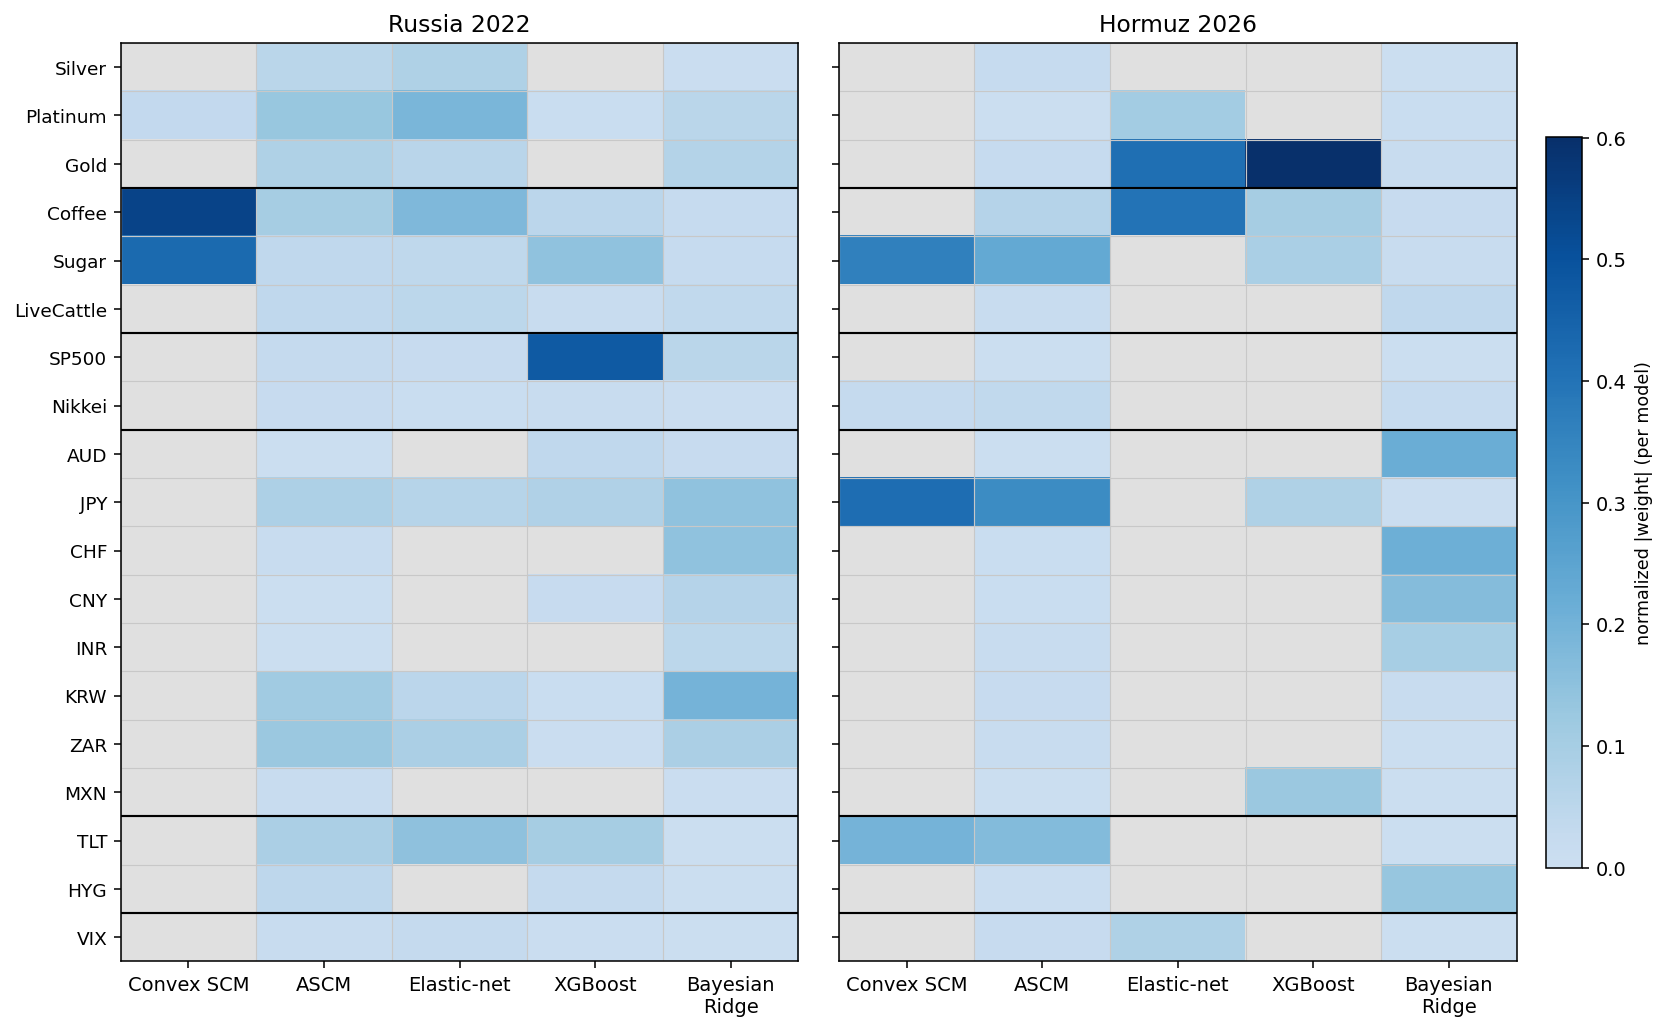
\includegraphics[width=\textwidth]{figures/donor_importance_heatmap.png}

\smallskip
\begin{minipage}{\textwidth}
\footnotesize \textit{Notes.} Each cell is a donor's weight in one model, taken in
absolute value and normalised to sum to one within that model; darker is larger, grey is
an unused (zero-weight) donor. Rows are the 19-donor shared pool grouped by category;
columns are the five estimators. The Bayesian ridge is shown for completeness but is
excluded from the consensus weight used in the text, as its coefficients are not
comparable selection weights (Appendix~\ref{app:bsts}). \textit{Source:}
\texttt{scripts/donor\_contribution\_analysis.py}.
\end{minipage}
\end{figure}

How a donor contributes sorts into two descriptive roles, each visible as a row of
Figure~\ref{fig:donorroles}.
\begin{itemize}
\item \textbf{Trend carriers} carry the largest donor weights, so their combination sets
  the synthetic's slow level path. Membership here follows the weight rather than a level
  correlation, since a linear correlation misses donors that contribute through more than
  straight-line co-movement. For Russia the carriers (Coffee, Sugar and the S\&P~500) climb
  alongside Brent. For Hormuz, Brent drifts down through 2024--25 while Gold and Coffee
  rise, so the synthetic reproduces the decline by loading donors that move the opposite
  way, and the yen, the second-heaviest donor, stays almost flat and anchors the level.
\item \textbf{Late divergers} sit on the pool's common factor at \T{} and then peel away over the post-window, shown in the bottom row where each line leaves zero after the cutoff. The role is defined by this behaviour and then attributed to a cause donor by
  donor, and the row plots only the divergers that also carry weight, since a donor that
  decouples but is never loaded cannot move the estimate. For Russia the weight sits on the
  Asian currencies, the yen and the Korean won, which the Fed tightening cycle pulled away
  from the rest of the pool from March 2022. Because the Bayesian ridge loads these
  currencies far more heavily than the other models, with convex SCM putting no weight on
  them at all, their post-event divergence falls mainly on its synthetic, which is what
  makes the Bayesian ridge the Russia outlier in Table~\ref{tab:headline}. The renminbi and
  rupee decouple further still
  on the discounted-crude terms-of-trade channel audited in Section~\ref{sec:donoraudit},
  but the models barely load them, so their divergence is left out of the figure and does
  not reach the gap. For Hormuz the single weighted diverger is Gold, falling away on its
  post-strike safe-haven bid.
\end{itemize}

\begin{figure}[h]
\centering
\caption{Donor paths by contribution role.}
\label{fig:donorroles}
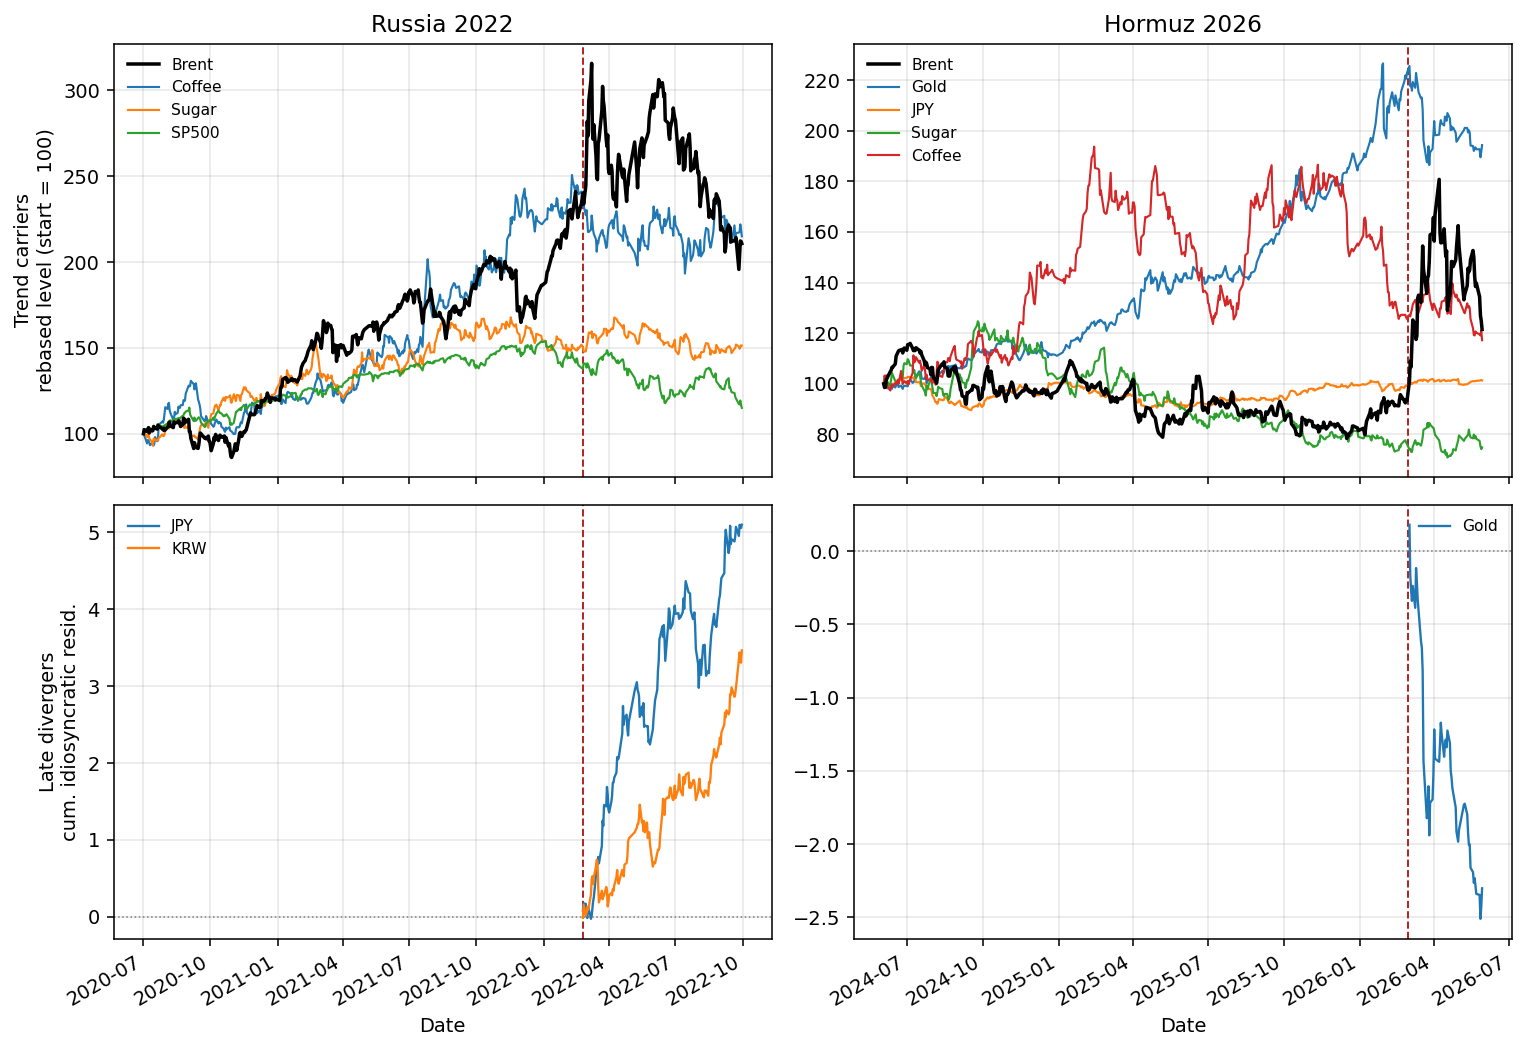
\includegraphics[width=\textwidth]{figures/donor_roles.png}

\smallskip
\begin{minipage}{\textwidth}
\footnotesize \textit{Notes.} Rows are the two roles and columns are the two events. The
dashed red line marks $T_0$. Trend carriers (top) are the highest-weight donors per event,
each rebased to 100 at the pre-window start. For Russia they co-move with Brent in levels,
while for Hormuz the heaviest movers (Gold, Coffee) run inversely as Brent drifts down and
the yen sits almost flat as a level anchor. Late divergers (bottom) are the weighted donors
that also decouple late, plotted as the standardised cumulative residual of the donor's
return on a leave-one-out, Brent-free common factor. Each sits near zero at $T_0$ and
decouples afterward. Donors with a large residual but negligible weight (CNY and INR) are
omitted because the models do not load them. The per-donor weights and diagnostics behind both rows are in
Appendix~\ref{app:donorweights}. Generated by \texttt{thesis/make\_figures.py}.
\end{minipage}
\end{figure}

What separates the models is how much weight they place on a few influential donors and how those donors behave after the event. The Hormuz estimate is driven by the models that
lean on Gold, and the Russia estimate by those that lean on the diverging currencies, so
the disagreement across models traces back to a handful of heavy donors rather than to
noise. This matters for the causal effect because the premium is the gap between actual
Brent and the synthetic, and that gap is a clean counterfactual only while the donors hold
their pre-event relationship to Brent. Once a loaded donor decouples after \T{}, the part
of the synthetic resting on it stops standing in for Brent and the donor's own drift leaks
into the estimated effect, growing as the window lengthens. For Russia the currencies drift
in the conservative direction, lifting the synthetic and trimming the measured premium, so
the contamination works against a large effect rather than inventing one. This is why the
ensemble takes the median and why the Russia full-window gap is read as the more
contaminated of the two estimates. The per-donor diagnostics are in
Appendix~\ref{app:donorweights}.

\subsection{Inference: the in-space placebo}
Table~\ref{tab:placebo} and Figure~\ref{fig:placebo} report the in-space placebo. For
\textbf{Hormuz} the result is as strong as the test allows. Brent ranks first among all
placebo units under every model and both donor pools, with a post/pre RMSPE ratio between
6.9 and 10.2 that exceeds every donor's, so the permutation $p$-value sits at the
attainable floor, 0.050 in the 19-donor pool and 0.030 in the 32-donor pool. For
\textbf{Russia} no model reaches the floor, and XGBoost comes closest at $p=0.20$. The
reason is mechanical. The volatile 2020--22 pre-period gives the donors large pre-period
RMSPE as well, which widens the placebo distribution and lowers the test's power. This is a
known low-power property of the in-space placebo under a volatile pre-period
\citep{abadie2010}, not evidence of a small effect, and we validate Russia's magnitude
independently below.

\begin{table}[h]
\centering
\caption{In-space placebo: permutation $p$-values and Brent's post/pre RMSPE ratio.}
\label{tab:placebo}
\begin{threeparttable}
\small
\begin{tabular}{@{}llrrr@{}}
\toprule
Event & Model & $p$ (19-donor) & $p$ (32-donor) & Brent ratio \\
\midrule
Russia & best of five (XGBoost) & 0.20 & 0.15 & 7.75 \\
\addlinespace
Hormuz & Convex SCM     & \textbf{0.050} & \textbf{0.029} & 6.93 \\
Hormuz & Augmented SCM  & \textbf{0.050} & \textbf{0.029} & 8.45 \\
Hormuz & Elastic net    & \textbf{0.050} & \textbf{0.029} & 8.53 \\
Hormuz & XGBoost        & \textbf{0.050} & \textbf{0.029} & 10.19 \\
Hormuz & Bayesian ridge & \textbf{0.050} & \textbf{0.029} & 10.24 \\
\bottomrule
\end{tabular}
\begin{tablenotes}[flushleft]
\footnotesize
\item \textit{Notes.} Floor $=1/(N{+}1)$: 0.050 (19-donor pool), 0.030 (32-donor pool).
\end{tablenotes}
\end{threeparttable}
\end{table}

\begin{figure}[h]
\centering
\caption{In-space placebo for Hormuz (convex SCM).}
\label{fig:placebo}
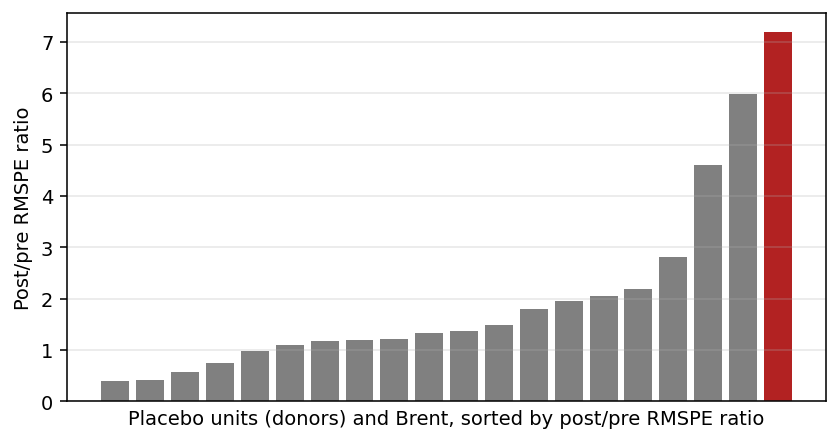
\includegraphics[width=0.72\textwidth]{figures/placebo_hormuz.png}

\smallskip
\begin{minipage}{0.72\textwidth}
\footnotesize \textit{Notes.} Each bar is one unit's post/pre RMSPE ratio. Brent (red) is
the largest and ranks first among all 19 placebo units, so the permutation test rejects at
the attainable floor.
\end{minipage}
\end{figure}

\subsection{Robustness}
\paragraph{Russia magnitude and external validation.} Because Russia is a known event, we
validate its magnitude against the EIA's last two pre-invasion Short-Term Energy Outlook
forecasts, issued before 24 February 2022. These forecasts are an independent structural
counterfactual that shares no information path with the SCM. Over the identical 151-day
window the ensemble-median synthetic mean of \$88.6 sits within \$3.6 of the STEO
February 2022 forecast of \$84.9, and three of five models bracket the STEO anchor to
within \$4. Two independent methods landing on nearly the same counterfactual is strong
evidence that the SCM does not produce an implausible path.

\paragraph{Post-window horizon sensitivity.} Figure~\ref{fig:sensitivity} reports the gap
at 1, 2, 3, and 6-month and full horizons. The two events show opposite and diagnostic
profiles. Russia declines with horizon, from about 31\% to 22\%, which is the signature of
delayed contamination as second-round war channels switch on through 2022 and pull the
synthetic up. The full-window figure is therefore conservative, and the
least-contaminated one-month estimate is about 31\%. Hormuz rises and then eases, from
about 46\% to 59\% and back to 56\%, which is the opposite of attenuation. The chokepoint
premium builds in and holds, and the slight easing at the full horizon reflects Brent's
partial mid-June pullback that appears once we extend the window to the latest data. The
same diagnostic declining for Russia and rising for Hormuz shows that it is not a
mechanical artefact.

\begin{figure}[h]
\centering
\caption{Ensemble-median gap by post-event horizon.}
\label{fig:sensitivity}

\includegraphics[width=0.78\textwidth]{figures/postwindow_sensitivity.png}

\smallskip
\begin{minipage}{0.78\textwidth}
\footnotesize \textit{Notes.} The shaded band is the IQR across models. Russia attenuates
with horizon, the delayed-contamination signature, while Hormuz rises and then plateaus as
the premium builds in and holds.
\end{minipage}
\end{figure}

\paragraph{Leave-one-donor-out.} Dropping each weighted donor in turn leaves the focal
Hormuz estimate tight around its baseline across all models (convex 51.2 to 59.3, ASCM
54.6 to 60.5, elastic 55.2 to 62.2, XGBoost 51.6 to 57.7\%), so no single donor drives the
result. For Russia we report the ensemble-median range rather than every model, because
Russia's wider spread comes from the simplex models' reliance on a few soft-commodity
donors, the same concentration that drives the contamination finding below. Read that way,
the wider Russia range (for example convex 32.8 to 59.6\%) is itself a symptom of the
donor-quality issue rather than a separate concern.

\paragraph{Cross-event weight stability.} As an exploratory probe rather than a validation
test, we apply the weights fitted on one event to the other event's window and read how far
the pre-period fit degrades. The transfer is weak, and that weakness is informative. Only
convex SCM transfers to a clearly positive Hormuz premium, at 25.3\% with a degraded but
non-pathological pre-fit, while the other models move toward or below zero with pre-fit
errors many times their independent level (Table~\ref{tab:transfer}). The reason is that
the two pre-periods are different factor regimes. Russia's 2020--22 pre-period is shaped by
the COVID recovery and the onset of Fed tightening, whereas Hormuz's 2024--26 pre-period is
a calmer disinflation regime, so the donor-to-Brent loadings that the weights encode do not
carry across. The models that fail hardest are the ones that load most on currencies, and
the dollar and emerging-market FX relationships shifted most between the two regimes.
Extending the Hormuz window through the June pullback widens the regime gap further. We
therefore read the transfer as weak and convex-only corroboration that some positive
premium survives a change of regime, and as direct evidence that fitting each event
separately is the correct choice, not as confirmation of the level.

\begin{table}[h]
\centering
\caption{Cross-event weight stability probe: Russia-fitted weights applied to Hormuz.}
\label{tab:transfer}
\begin{threeparttable}
\small
\begin{tabular}{@{}lrrrr@{}}
\toprule
Model & Indep.\ gap (\%) & Transf.\ gap (\%) & Indep.\ RMSPE & Transf.\ RMSPE \\
\midrule
Convex SCM     & 55.9 & 25.3   & 0.066 & 0.336 \\
Augmented SCM  & 56.8 & $-0.8$  & 0.066 & 0.467 \\
Elastic net    & 56.6 & $-68.6$ & 0.054 & 1.513 \\
XGBoost        & 51.2 & $-44.1$ & 0.053 & 0.928 \\
Bayesian ridge & 43.0 & $-100.0$ & 0.037 & 18.567 \\
\bottomrule
\end{tabular}
\begin{tablenotes}[flushleft]
\footnotesize
\item \textit{Notes.} Independent and transferred pre-period RMSPE in log units.
\end{tablenotes}
\end{threeparttable}
\end{table}

\paragraph{Na\"ive counterfactual floor.} We compare the SCM against donor-free univariate
counterfactuals built only from Brent's own past (Table~\ref{tab:naive}), and the
comparison yields three findings. First, the SCM adds value. It sits about 13 points above
the trend-free random-walk null for Russia and about 7 points above it for Hormuz, so the
donor machinery extracts something that extrapolating Brent's own series cannot. Second,
and most telling, the naive bias flips sign across the two events purely because the
pre-window trend sign differs. The linear trend extrapolates Russia's recovery rally upward
and returns an implausible negative full-window gap of about $-4\%$, yet the same method
extrapolates Hormuz's mild downtrend and inflates the gap to about 71\%. A counterfactual
built from one series alone is therefore regime-fragile in a way the donor-based SCM is not.
Third, for Russia the SCM and the trend extrapolation sit on opposite sides of the truth.
The SCM leans high, as the contamination analysis below confirms, and the trend
extrapolation leans low, so the two bracket the real value, with the random-walk null at
$+8.7\%$ the most defensible naive point. The naive floor and the contamination analysis
thus corroborate each other, one from a donor-free direction and one from a donor-based one.

\begin{table}[h]
\centering
\caption{SCM vs.\ na\"ive univariate counterfactuals, full-window gap (\%).}
\label{tab:naive}
\begin{threeparttable}
\small
\begin{tabular}{@{}lrrrr@{}}
\toprule
Event & SCM median & RW flat & RW drift & Lin.\ trend \\
\midrule
Russia & 22.0 & 8.7  & $-6.9$ & $-4.2$ \\
Hormuz & 55.9 & 48.9 & 49.8   & 70.9   \\
\bottomrule
\end{tabular}
\begin{tablenotes}[flushleft]
\footnotesize
\item \textit{Notes.} RW flat and RW drift are the random-walk carry and the drifted random walk; Lin.\ trend is the linear pre-trend extrapolation. An AIC-selected ARIMA reduces to a driftless random walk for both events (RW flat column).
\end{tablenotes}
\end{threeparttable}
\end{table}

\paragraph{Sign of the contamination bias.} This last check is a deliberately naive and
directional diagnostic, not a structural correction. It does not prove that the donors are
clean. It asks a narrower question. If some contamination remains despite the audit and the
break tests, which way would it bias the estimate? We answer it with equation~\eqref{eq:bias}
and a Brent-free reference, and the two events give opposite and informative answers. For
\textbf{Hormuz}, where every other check already supports a stable estimate, any residual
contamination has a small negative sign, between about $-1$ and $-8\%$. The reading is
reassuring in one direction. If the estimate is biased at all, it is biased downward, so the
true premium is at least as large as we report and the headline is conservative. For
\textbf{Russia} the sign reverses and the bias is large and positive, on the order of
$+13$ to $+21\%$. The reason is economic. The high-price and risk-off environment of 2022
depressed the demand-cyclical donors, the equities, metals, and soft commodities, relative
to the safe-haven and currency donors, so the synthetic built from them sits too low and the
gap reads too high. The bias concentrates in the low-reliability soft-commodity donors, and
splitting donors by pre-window factor $R^2$ confirms that most of it sits in the
low-reliability group rather than in the donors that track the common factor well. The
conclusion is asymmetric. Contamination is conservative for the focal Hormuz estimate and
inflates the Russia full-window number, so Russia's magnitude validation rests on the early
and peak window, where the \$95$\to$\$130 move is recovered, and not on the attenuated
full-window average.

\subsection{Interpretation}
The 2026 Hormuz chokepoint premium is roughly \SI{56}{\percent} of Brent's no-event level
over the first three and a half months, and the estimate is stable. It holds across all
five estimators and clears the validation battery of Section~\ref{sec:methods}, with the
in-space placebo reaching its attainable floor as the strongest single result. The
contamination analysis adds a useful direction to this stability. If anything, the true
Hormuz premium is larger than our estimate, not smaller. The cross-event probe is the
weakest of the checks, and we lean on it only for the sign of the effect under a change of
regime, never for its level. We read the estimate as a complement to the structural
scenario estimates from energy institutions rather than a competitor to them. Those answer
the question of what price an assumed barrel shortfall implies, while the SCM answers what
price gap the observed cross-asset co-movement implies, and the two questions inform
different parts of a policy response. For the levers set out in Section~\ref{sec:intro},
reserve releases, monetary pass-through, and fiscal buffers, the relevant input is the
integrated path-level premium, and the estimate here supplies it together with an auditable
identification argument.

